\documentclass{beamer}

\usetheme{Antibes}

%\usetheme{split}
%\usetheme{Madrid}
%\usetheme{Berkeley}
\usecolortheme[RGB={120,0,0}]{structure}
\setbeamertemplate{blocks}[rounded][shadow=true]
\setbeamertemplate{footline}{\hfill\insertframenumber{}\hspace*{0.2cm}\vspace*{0.2cm}}
\usepackage[utf8]{inputenc}   % pacote para acentuao
\usepackage{graphicx}
\usepackage{subcaption}

%\usepackage[latin1]{inputenc}

\beamertemplateballitem
\beamertemplatenavigationsymbolsempty

\begin{document}

\title{Assessing the Computation and Communication Overhead of Linux Containers for HPC Applications}
\author{
\large 
Guilherme Rezende Alles\\
Lucas Mello Schnorr\\
Alexandre Carissimi\\
\small
\vspace*{0.5cm}
Instituto de Informática\\
Universidade Federal do Rio Grande do Sul
}
\logo{
\includegraphics[scale=0.3]{inf}}
\date{21 de Junho de 2018}

\frame{\titlepage}

\frame{\frametitle{Why is this relevant?}
    \begin{itemize}
        \item Scientists should spend their time researching, and not figuring out execution environment specifics
        \item Dependency management hell
        \item Reproducible research should be the default, not a "plus"
    \end{itemize}
    
    \begin{itemize}
        \item Solution? Virtual machines! But...
        \begin{itemize}
            \item Requires a hypervisor, which is probably cumbersome and not always installed on the host
            \item Operating system images are large and can take a while to build and distribute
            \item \textbf{Overhead}
        \end{itemize}
    \end{itemize}
}

\frame{\frametitle{Why is this relevant?}
    There is a workaround: Linux Containers!
    \begin{itemize}
        \item No hypervisor, thus lower overhead
        \item Images take much less space
        \item Requirement is the Linux Kernel, which most HPC Clusters already run
        \item Provides flexibility that can yield performance gains at a small development cost
    \end{itemize}
}

\frame{\frametitle{Motivation & Objectives}
    
}

\frame{
    \begin{itemize}
        \item table of contents
    \end{itemize}
}

\frame{\frametitle{Linux Containers}
    \begin{itemize}
        \item Operating System level virtualization
        \item Resource control and isolation build into the Linux Kernel
        \item Cgroups and Namespaces API
        \item Complex operation
    \end{itemize}
    \centering
    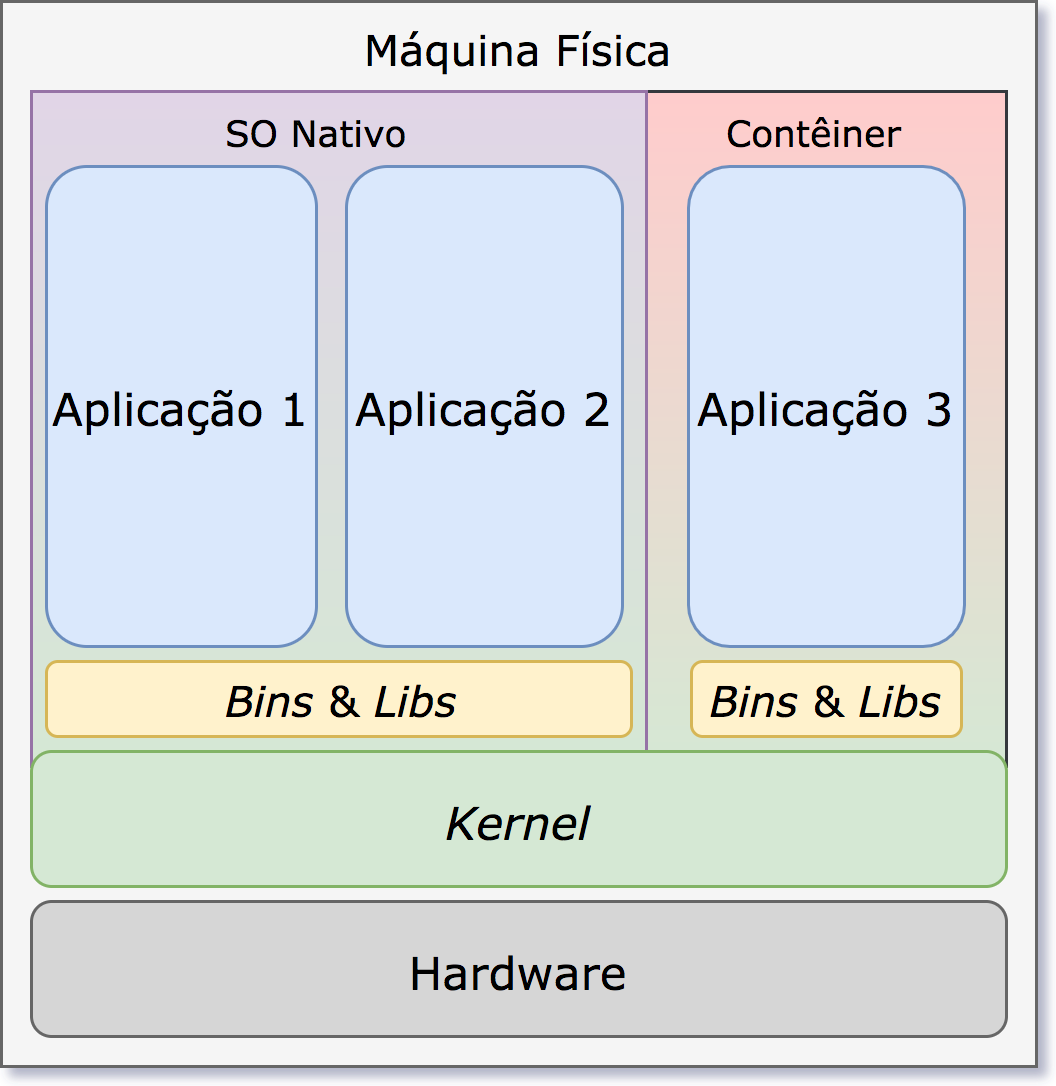
\includegraphics[width=.2\textwidth]{conteineres.png}\\
    \footnotesize(translate this figure, probably enhance it)
}

\frame{\frametitle{docker}
    \begin{itemize}
        \item Main use case: microservice virtualization
        \item Widely used in the industry
        \item Easily found in cloud infrastructure providers such as AWS, GCP and Azure
        \item philosophy: enforce the virtualization of every namespace provided by the Linux Kernel
        \begin{itemize}
            \item \textbf{User}, file system, \textbf{network}, IPC, pid
            \item Implications on the use case (elaborate in that)
        \end{itemize}
    \end{itemize}
}

\frame{\frametitle{singularity}
    \begin{itemize}
        \item Linux Containers for HPC
        \item Alternative to Docker drawbacks for shared environments
        \item Aims for a secure container environment that can be installed in clusters
        \item philosophy: only virtualize the necessary namespaces, while everything else is kept optional.
        \begin{itemize}
            \item \textbf{file system}
        \end{itemize}
    \end{itemize}
}

\frame{\frametitle{testbed}
    \begin{itemize}
        \item Grid5000's Graphene clusters
        \begin{itemize}
            \item Intel Xeon X3340, 4 cores @ 2.53GHz
            \item 16GB DDR3 RAM
            \item Gigabit Ethernet interconnect
        \end{itemize}
        \vspace*{0.5cm}
        \item Debian 9 (\textit{stretch}) Linux
        \begin{itemize}
            \item Singularity containers running on top of the native environment
            \item Docker containers connected through Docker Swarm \textit{overlay}
        \end{itemize}
    \end{itemize}
}

\frame{\frametitle{workload}
    \begin{itemize}
        \item NAS Parallel Benchmarks
        \begin{itemize}
            \item Synthetic workload for baseline purposes
            \item EP (\textit{embarrassingly parallel}) Kernel
            \begin{itemize}
                \item CPU bound scenario
                \item Low communication between workers
                \item Workload size B
            \end{itemize}
        \end{itemize}
        \vspace*{0.3cm}
        \item Ondes3D
        \begin{itemize}
            \item Seismic waves propagation simulation
            \item Load imbalance, frequent communication
            \begin{itemize}
                \item Workload: default test case + Ligurian
            \end{itemize}
        \end{itemize}
        \vspace*{0.3cm}
        \item Ping-Pong benchmark
        \begin{itemize}
            \item Network latency
        \end{itemize}
    \end{itemize}
}

\frame{\frametitle{results}
    \begin{itemize}
        \item NAS EP raw results
        \item NAS EP computed overhead against native
    \end{itemize}
}

\frame{\frametitle{results}
    \begin{itemize}
        \item Ondes3D raw results
        \item Ondes3D computed overhead against native
    \end{itemize}
}

\frame{\frametitle{results}
    \begin{itemize}
        \item Ping-pong raw results
        \item Ping-pong overhead against native (???)
    \end{itemize}
}

\end{document}